\documentclass[submission,copyright,creativecommons]{eptcs}
\providecommand{\event}{TTC 2015} % Name of the event you are submitting to
\usepackage{breakurl}             % Not needed if you use pdflatex only.
\usepackage{flafter}
\usepackage{listings}
\usepackage{graphicx}
\usepackage{url}
\usepackage{color}

%ATL language highlighting
\lstdefinelanguage{atl}
{
  sensitive=true,
  morecomment=[l]{--},
  morestring=[b]',
  classoffset=0,
  morekeywords={module, create, from, to, using, mapsTo, rule, helper, refining,
                context, def, if, then, else, endif, library, and, or, not, query, 
                do, endpoint, entrypoint, lazy, unique, nodefault, for, in, self,
                thisModule, uses, let},
  classoffset=1,
  morekeywords={OclAny,Integer,Real,String,Boolean,Collection,Bag,Set,OrderedSet,
                Sequence,Map,Tuple,TupleType}
}

%SimpleGT language highlighting
\lstdefinelanguage{simplegt}
{
  sensitive=true,
  morecomment=[l]{--},
  classoffset=0,
  morekeywords={module, import, transform, from, to, abstract, rule, before, 
                def, if, then, else, endif, and, or, not, lazy, unique, default,
                in, self, uses, env, single, context, static, let, metamodel},
  classoffset=1,
  morekeywords={OclAny,Integer,Real,String,Boolean,Collection,Bag,Set,OrderedSet,
                Sequence,Map,Tuple,TupleType,Env}
}

\definecolor{commentgreen}{rgb}{0.0, 0.4, 0.1}
\definecolor{commentblue}{rgb}{0.0, 0.1, 0.4}
\definecolor{typegreen}{rgb}{0.0, 0.6, 0.0}
\definecolor{keywordred}{rgb}{0.4, 0.0, 0.1}

%Standard listing style
\lstset{
  numbers=left,
  numberstyle=\tiny,
  stepnumber=1,
  numbersep=5pt,
  tabsize=2,
  basicstyle=\scriptsize\tt,
  commentstyle=\scriptsize\tt\color{commentblue},
  stringstyle=\scriptsize\tt\color{blue},
  classoffset=0,
  keywordstyle=\scriptsize\tt\bf\color{keywordred},
  classoffset=1,
  keywordstyle=\scriptsize\tt\color{typegreen},
  classoffset=0 % restore default
}

\title{The {ATL/EMFTVM} Solution to the Train Benchmark Case for {TTC2015}}
\author{Dennis Wagelaar
\institute{HealthConnect\\
Vilvoorde, Belgium}
\email{dennis.wagelaar@healthconnect.be}
}
\def\titlerunning{The {ATL/EMFTVM} Solution to the Train Benchmark Case for {TTC2015}}
\def\authorrunning{D. Wagelaar}
\begin{document}
\maketitle

\begin{abstract}
This paper describes the ATL/EMFTVM solution of the TTC 2015 Train Benchmark Case. The Train Benchmark Case consists of several model validation and model repair tasks, all of which are run again increasing model sizes in order to measure the performance of each solution for the case. A complete solution for all tasks is provided, and is discussed with regard to the three provided evaluation criteria: Correctness and Completeness of Model Queries and Transformations, Applicability for Model Validation, and Performance on Large Models.
\end{abstract}

\section{Introduction}
\label{sec:intro}

This paper describes the ATL/EMFTVM~\cite{journal/scp/Jouault2008} solution of the TTC 2015 Train Benchmark Case~\cite{conf/ttc/Szarnyas2015}. The Train Benchmark Case consists of several model validation and model repair tasks, all of which are run again increasing model sizes in order to measure the performance of each solution for the case. A complete solution for all tasks is provided, and is available as a GitHub fork of the original assignment\footnote{\url{https://github.com/dwagelaar/trainbenchmark-ttc}}.

The remainder of this paper is structured as follows: section~\ref{sec:atl} describes the ATL transformation tool and its features that are relevant to the case. Section~\ref{sec:solution} describes the solution to the case, and section~\ref{sec:eval} concludes this paper with an evaluation.

\section{ATL}
\label{sec:atl} 

ATL is a rule-based, hybrid model transformation language that allows declarative as well as imperative transformation styles. For this TTC solution, we use the new EMF Transformation Virtual Machine (EMFTVM)~\cite{conf/models/Wagelaar2011}. EMFTVM includes a number of language enhancements, as well as performance enhancements. For this TTC case, specific performance enhancements are relevant. Each of these enhancements is described briefly in the following subsections.

\subsection{JIT compiler}

EMFTVM includes a Just-In-Time (JIT) compiler that translates EMFTVM bytecode to Java bytecode. EMFTVM bytecode instructions are organised in \emph{code blocks} (see Fig.~\ref{fig:emftvm-rules}). Code blocks are executable lists of instructions, and have a number of local variables and a local stack space. Code blocks are used to represent operation bodies, field initialisers, rule guards, and rule bodies. Code blocks may also have nested code blocks, which effectively represent \emph{closures}\footnote{\url{http://en.wikipedia.org/wiki/Closure\_(computer_programming)}}. EMFTVM records how often each code block is executed, as well as some execution metadata, such as which methods were dispatched in each virtual method call. When a code block is executed more often than a predefined threshold, the JIT compiler triggers, and will generate a Java bytecode equivalent for the EMFTVM code block. The JIT compiler provides the best performance improvement for large and complex code blocks.

\begin{figure}[ht]
\centerline{
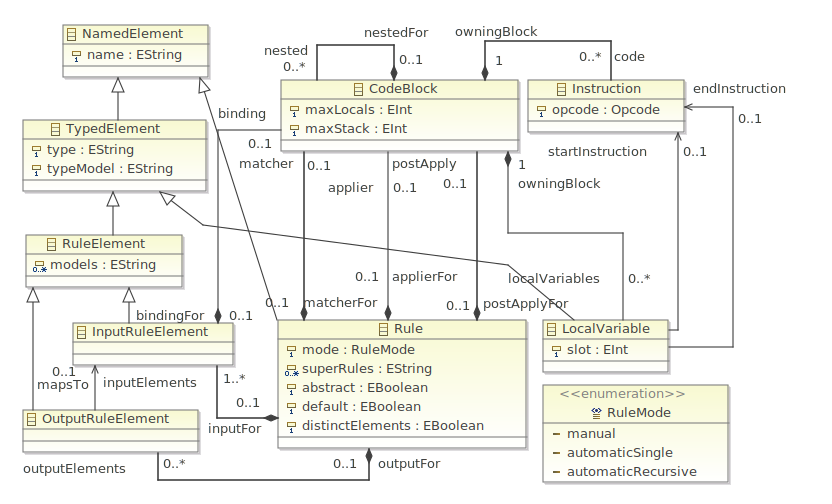
\includegraphics[width=12cm]{figures/emftvm-rules-stripped}}
\caption{Structure of EMFTVM rules and code blocks}
\label{fig:emftvm-rules}
\end{figure}

\subsection{Lazy evaluation}

EMFTVM includes an implementation of the OCL 2.2 standard library~\cite{omg/ocl22}, and employs lazy evaluation for the collection operations\footnote{\url{https://wiki.eclipse.org/ATL/EMFTVM\#Lazy\_collections}} (e.g. \texttt{select}, \texttt{collect}, \texttt{flatten}, \texttt{isEmpty}, etc.). That means you can invoke operations on the collections, but those operations will not be executed until you actually evaluate the collection. Also, collection operations will only be evaluated partially, depending on how much of the collection you evaluate. To illustrate how this works, look at the example code in Listing~\ref{lst:lazy}. The \texttt{lazytest} query invokes "collect" on a Sequence of all numbers from 0 to 100, and replaces each value in the Sequence by its squared value. Finally, we're only interested in the last value of the changed Sequence. \texttt{collect} returns a lazy Sequence, which is just waiting to be evaluated. Only when "last" is invoked on the lazy Sequence will the Sequence invoke the "expensive" operation on the last element of the input Sequence. As a result, \texttt{square} is only invoked once.

\lstset{language=atl}
\begin{lstlisting}[float=htb, caption={Lazy collections in ATL}, label=lst:lazy, captionpos=b, frame=tb, belowskip=-10pt]
query lazytest = Sequence{0..100}->collect(x | x.square())->last();

helper context Integer def : square() : Integer =
	(self * self).debug('square');
\end{lstlisting}

In addition, short-circuit evaluation is applied to boolean expressions (i.e. \textbf{and}, \textbf{or}, and \textbf{not}). While this may not be a desirable semantics for OCL in general, it is advantageous for using OCL as a navigation language: only the relevant parts of the model are navigated. Lazy evaluation provides the best performance improvement when only consuming a small part of a string of collection operations (e.g. \texttt{list->reject(x | x.attr.oclIsUndefined())->collect(x | x.attr)->first()}). Short-\\circuit evaluation prevents having to use (nested) \texttt{if-then-else-endif} blocks everywhere.

\subsection{Caching of model elements}

Model transformations usually look up model elements by their type or meta-class. In the Eclipse Modeling Framework (EMF)~\cite{book/Budinsky03}, this means iterating over the entire model and filtering on element type. Often, an element look up by type is made repeatedly on the same model (especially when doing recursive, in-place transformation\footnote{\url{https://code.google.com/a/eclipselabs.org/p/simplegt/}}). In the case of this benchmark, the same query/transformation is run multiple times on the same model. For this reason, EMFTVM keeps a cache of model elements by type for each model. This cache is automatically kept up to date when adding/removing model elements through EMFTVM. The cache is built up lazily, which means that a full iteration over the model, looking for a specific element type, must have taken place before the cache is activated for that element type. This prevents a build up of caches that are never used.

\section{Solution Description}
\label{sec:solution}

The Train Benchmark Case involves first querying a model for constraint violations, and then repairing some of those constraint violations that are randomly selected by the benchmark framework. This means that the matching phase and the transformation phase, which are normally integrated in ATL, are now separated by the benchmark framework. The framework first launches the matching phase, and collects the found matches. After that, it randomly selects a number of matches, and feeds them into the transformation phase.

ATL provides a \textbf{query} construct that allows one to query the model using OCL. The resulting values are returned by the ATL VM. The selected matches are fed back into the ATL VM through a helper attribute, specified in the framework repair transformation module shown in Listing~\ref{lst:repair}. Note that the ATL query returns a \emph{lazy} collection, which is just waiting to be evaluated. The benchmark framework compensates for this by copying all values of the returned lazy collection into a regular \texttt{java.util.ArrayList}, which triggers evaluation. This ensures that the performance measurements are valid.

\lstset{language=atl}
\begin{lstlisting}[float=htb, caption={Framework repair transformation module in ATL}, label=lst:repair, captionpos=b, frame=tb, belowskip=-10pt]
module Repair;
create OUT: RAILWAY refining IN: RAILWAY;

--- Helper attribute that holds the matches to transform.
--- Injected from outside the transformation.
helper def : matches : Collection(OclAny) = Sequence{};

--- Base implementation of the Repair rule that does nothing.
lazy rule Repair {
	from
		s: OclAny
}

--- Applies the Repair rule to all matches.
endpoint rule Main() {
	do {
		for (s in thisModule.matches) {
			thisModule.Repair(s);
		}
	}
}
\end{lstlisting}

The Repair transformation module contains a helper attribute \texttt{matches}, which is used to inject the matches selected by the benchmark framework. Furthermore, it contains a lazy rule \texttt{Repair}, which does nothing in this framework transformation. The \texttt{Repair} rule is invoked by every element in \texttt{matches} by the \texttt{Main} endpoint rule. The \texttt{Main} endpoint rule is automatically invoked. Normally, ATL transformations use matched rules that are automatically triggered for all matching elements in the input model(s). However, this benchmark requires the elements to transform to be set explicitly. Hence the need for this framework transformation module. All specific repair transformation modules are \emph{superimposed}~\cite{journal/sosym/Wagelaar2009} onto the framework transformation module, and redefine the \texttt{Repair} rule. This means that for each task we only need to define an ATL query and a \texttt{Repair} rule. The Java code in the benchmark plug-in for ATL is made up of a base class \texttt{ATLBenchmarkCase} that provides the generic logic for:

\begin{enumerate}
\item instantiating a query VM, a transformation VM, and loading the metamodels (\texttt{init});
\item loading the models (\texttt{read});
\item performing the query phase of the benchmark (\texttt{check});
\item performing the transformation phase of the benchmark (\texttt{modify}).
\end{enumerate}

Each specific task subclasses the \texttt{ATLBenchmarkCase} class, but only has to override the \texttt{init} method. The overridden \texttt{init} does all of the superclass \texttt{init}, but also loads the ATL transformation bytecode into the query VM and the transformation VM.

\subsection{Task 1: PosLength}

The PosLength task consists of a query that checks for Segments with a length less than or equal to zero, and a repair transformation that updates the length attribute of the segment in the match to \texttt{−length+1}. 

Listing~\ref{lst:poslength} shows the ATL query for Poslength. It simply collects all Segment instances with a length of zero or smaller.

\lstset{language=atl}
\begin{lstlisting}[float=htb, caption={PosLength query in ATL}, label=lst:poslength, captionpos=b, frame=tb, belowskip=-10pt]
query PosLength = RAILWAY!Segment.allInstances()->select(s | s.length <= 0);
\end{lstlisting}

Listing~\ref{lst:poslengthrepair} shows the ATL repair transformation module for Poslength. It imports the framework Repair transformation module from Listing~\ref{lst:repair}, and redefines the \texttt{Repair} rule. As no new elements need to be created, and no implicit tracing of source elements to target elements is required, an imperative \textbf{do} block is used to make the required modification directly on the source element. The \texttt{<:=} assignment operator is used instead of the \texttt{<-} binding operator, such that the implicit source-to-target tracing is skipped.

\lstset{language=atl}
\begin{lstlisting}[float=htb, caption={PosLength repair transformation module in ATL}, label=lst:poslengthrepair, captionpos=b, frame=tb, belowskip=-10pt]
module PosLengthRepair;
create OUT: RAILWAY refining IN: RAILWAY;

uses Repair;

lazy rule Repair {
	from
		s: RAILWAY!Segment
	do {
		s.length <:= -s.length + 1;
	}
}
\end{lstlisting}

\subsection{Task 2: SwitchSensor}

The SwitchSensor task consists of a query that checks for Switches that are not connected to a Sensor, and a repair transformation that creates and connects a new Sensor. 

Listing~\ref{lst:switchsensor} shows the ATL query for SwitchSensor. It collects all Switch instances for which the sensor is not set.

\lstset{language=atl}
\begin{lstlisting}[float=htb, caption={SwitchSensor query in ATL}, label=lst:switchsensor, captionpos=b, frame=tb, belowskip=-10pt]
query SwitchSensor = RAILWAY!Switch.allInstances()->select(s | s.sensor.oclIsUndefined());
\end{lstlisting}

Listing~\ref{lst:switchsensorrepair} shows the ATL repair transformation module for SwitchSensor. This time, the \texttt{Repair} rule also contains a \textbf{to} section that creates a new Sensor instance \texttt{se}. In the \textbf{do} section, this Sensor is assigned to the sensor reference of the input Switch element.

\lstset{language=atl}
\begin{lstlisting}[float=htb, caption={SwitchSensor repair transformation module in ATL}, label=lst:switchsensorrepair, captionpos=b, frame=tb, belowskip=-10pt]
module SwitchSensorRepair;
create OUT: RAILWAY refining IN: RAILWAY;

uses Repair;

lazy rule Repair {
	from
		s: RAILWAY!Switch
	to
		se: RAILWAY!Sensor
	do {
		s.sensor <:= se;
	}
}
\end{lstlisting}

\subsection{Task 3: SwitchSet}

The SwitchSet task consists of a query that checks for Routes that are not connected to a Sensor, which have a semaphore that show the GO signal. Additionally, the route follows a switch position (p) that is connected to a switch (sw), but the switch position (p.position) defines a different position from the current position of the switch (sw.currentPosition). Furthermore, a repair transformation is provided, which sets the currentPosition attribute of the switch to the position of the switchPosition. 

Listing~\ref{lst:switchset} shows the ATL query for SwitchSet. The query collects Tuples of each match, where a match is defined by Route \texttt{r}, Semaphore \texttt{s}, SwitchPosition \texttt{p}, and Switch \texttt{sw}. A Tuple is created for each wrong SwitchPosition that was found for each Route with a ``GO'' signal. As one can see, Tuples allow for returning matches with multiple elements to the benchmark framework.

\lstset{language=atl}
\begin{lstlisting}[float=htb, caption={SwitchSet query in ATL}, label=lst:switchset, captionpos=b, frame=tb, belowskip=-10pt]
query SwitchSet = RAILWAY!Route.allInstances()
	->select(r | 
		not r.entry.oclIsUndefined() and r.entry.signal = #GO
	)->collect(r | r.follows
		->select(p | 
			not p.switch.oclIsUndefined() and p.switch.currentPosition <> p.position
		)->collect(p | 
			Tuple{r = r, s = r.entry, p = p, sw = p.switch}
		)
	)->flatten();
\end{lstlisting}

Listing~\ref{lst:switchsetrepair} shows the ATL repair transformation module for SwitchSet. The \texttt{Repair} rule takes the Tuple match as input element this time, and assigns the SwitchPosition's position to the Switch's currentPosition.

\lstset{language=atl}
\begin{lstlisting}[float=htb, caption={SwitchSet repair transformation module in ATL}, label=lst:switchsetrepair, captionpos=b, frame=tb, belowskip=-10pt]
module SwitchSetRepair;
create OUT: RAILWAY refining IN: RAILWAY;

uses Repair;

lazy rule Repair {
	from
		s : TupleType(
			r : RAILWAY!Route, 
			s : RAILWAY!Semaphore, 
			p : RAILWAY!SwitchPosition, 
			sw : RAILWAY!Switch)
	do {
		s.sw.currentPosition <:= s.p.position;
	}
}
\end{lstlisting}

\subsection{Extension Task 1: RouteSensor}

The RouteSensor task consists of a query that checks for Sensors that are connected to a Switch, but the Sensor and the Switch are not connected to the same Route. The repair transformation inserts the missing definedBy Sensors for the Route. 

Listing~\ref{lst:routesensor} shows the ATL query for RouteSensor. The query collects Tuples of each match, where a match is defined by Route \texttt{r}, SwitchPosition \texttt{p}, Switch \texttt{sw}, and Sensor \texttt{s}. A Tuple is created for each SwitchPosition connected to a Sensor that is not connected to the Route, for each Route that has Sensors connected to it. 

\lstset{language=atl}
\begin{lstlisting}[float=htb, caption={RouteSensor query in ATL}, label=lst:routesensor, captionpos=b, frame=tb, belowskip=-10pt]
query RouteSensor = RAILWAY!Route.allInstances()
	->select(r | r.definedBy->notEmpty())
	->collect(r |
		r.follows->select(p | 
			not p.switch.oclIsUndefined() and 
			not p.switch.sensor.oclIsUndefined() and
			r.definedBy->excludes(p.switch.sensor)
		)->collect(p | 
			Tuple{r = r, p = p, sw = p.switch, s = p.switch.sensor}
		)
	)->flatten();
\end{lstlisting}

Listing~\ref{lst:routesensorrepair} shows the ATL repair transformation module for RouteSensor. The \texttt{Repair} rule takes the Tuple match as input element, and adds the Sensor in the match to the Route's definedBy sensors.

\lstset{language=atl}
\begin{lstlisting}[float=htb, caption={RouteSensor repair transformation module in ATL}, label=lst:routesensorrepair, captionpos=b, frame=tb, belowskip=-10pt]
module RouteSensorRepair;
create OUT: RAILWAY refining IN: RAILWAY;

uses Repair;

lazy rule Repair {
	from
		s : TupleType(
			r : RAILWAY!Route, 
			p : RAILWAY!SwitchPosition, 
			sw : RAILWAY!Switch,
			s : RAILWAY!Sensor)
	do {
		s.r.definedBy <:= s.r.definedBy->including(s.s);
	}
}
\end{lstlisting}

\subsection{Extension Task 2: SemaphoreNeighbor}

The SemaphoreNeighbor task consists of a query that checks for Routes \texttt{r1} that have an exit Semaphore, and a Sensor \texttt{s1} connected to another Sensor \texttt{s2} -- defining another Route \texttt{r3} -- by two TrackElements \texttt{te1} and \texttt{te2}, for which there is no other Route \texttt{r2} that connects the same Semaphore and the other Sensor \texttt{s2}. Furthermore, a repair transformation is provided, which removes the exit Semaphore from Route \texttt{r1}.

Listing~\ref{lst:semaphoreneighborquery} shows the ATL query for SemaphoreNeighbor. The query uses a SimpleGT~\cite{conf/models/Wagelaar2011} transformation module to collect matches. SimpleGT is a minimal graph transformation language with embedded OCL support, and supports local search plans for pattern matching. Both SimpleGT and ATL compile to EMFTVM bytecode, and can hence be executed together as a single transformation. Experimentation has shown the EMFTVM local search support to be more performant than encoding the search plan directly in OCL. The pure ATL/OCL query alternative solution is given for reference purposes in Appendix~\ref{appendix:a}.

\lstset{language=atl}
\begin{lstlisting}[float=htb, caption={SemaphoreNeighborQuery in ATL}, label=lst:semaphoreneighborquery, captionpos=b, frame=tb, belowskip=-10pt]
query SemaphoreNeighbourQuery = thisModule.traces.getLinksByRule('Check', true).links
		->collect(l | Tuple{
			s = l.getSourceElement('s', true).object,
			r1 = l.getSourceElement('r1', true).object,
			r2 = l.getSourceElement('r2', true).object,
			s1 = l.getSourceElement('s1', true).object,
			s2 = l.getSourceElement('s2', true).object,
			te1 = l.getSourceElement('te1', true).object,
			te2 = l.getSourceElement('te2', true).object});

uses SemaphoreNeighbourCheck;
\end{lstlisting}

SimpleGT matches are recorded in the implicit trace model by EMFTVM. The ATL query reads the recorded traces using reflection, and creates OCL Tuples for each matching trace. Fig.~\ref{fig:emftvm-trace} shows a class diagram of the EMFTVM Trace metamodel, including the built-in operations. The root object of the trace model is a TraceLinkSet, which can be accessed from ATL using the built-in \texttt{thisModule.traces} helper attribute.

\begin{figure}[ht]
\centerline{
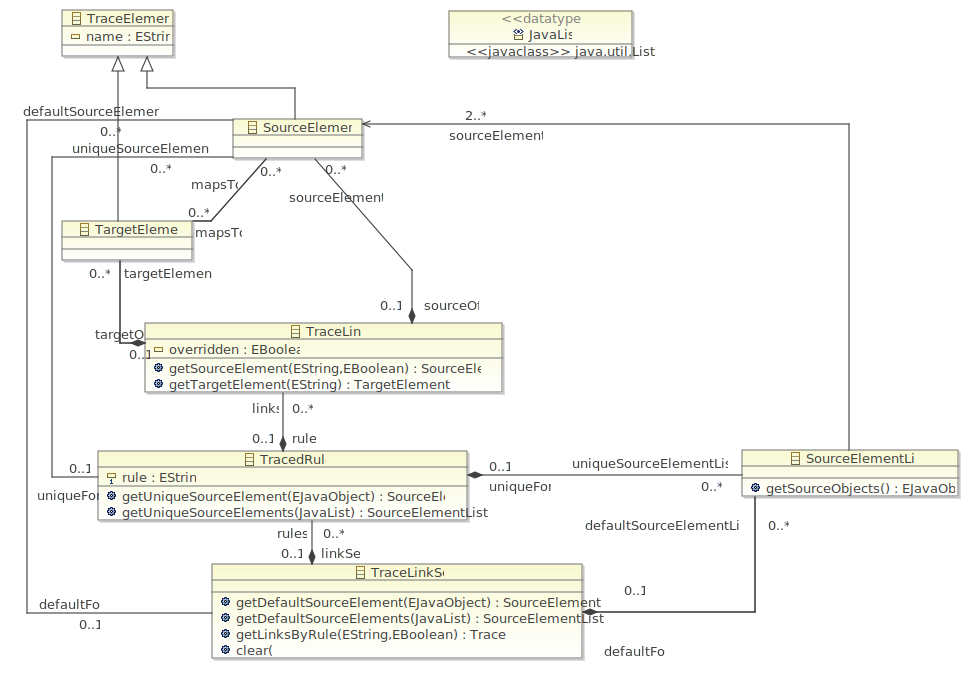
\includegraphics[width=15cm]{figures/trace}}
\caption{The EMFTVM Trace metamodel}
\label{fig:emftvm-trace}
\end{figure}

Listing~\ref{lst:semaphoreneighborcheck} shows the SimpleGT check transformation for SemaphoreNeighbor. It uses a ``single'' rule (i.e. one-shot, non-recursive matching) to match the required pattern. Whenever a navigation is possible from one element to the next, the SimpleGT compiler produces a local search expression to find the next element. EMFTVM will evaluate this local search expression whenever available instead of iterating over the entire model. There is one situation where direct navigation is not possible: finding Route \texttt{r2} from Sensor \texttt{s2}. To get around this problem, the \texttt{route} helper attribute is defined on the Sensor metaclass. This helper attribute retrieves the container object for the Sensor, as \texttt{Route::definedBy} is a containment reference. The \texttt{route} helper attribute can now be used in the Check rule to navigate from Sensor \texttt{s2} to all possible Routes \texttt{r2}. The \textbf{not} part in the rule represents a \emph{negative application condition} (NAC), which specifies a condition that may not occur in a valid match. A rule can have multiple \textbf{not} parts. SimpleGT requires you to specify a \emph{left-hand-side} (LHS) and \emph{right-hand-side} (RHS) for each rule, represented by the \textbf{from} and the \textbf{to} part, respectively. The LHS is always replaced by the RHS. Because we don't want the Check rule to change anything, we must repeat the LHS in the RHS to prevent it from being deleted.

\lstset{language=simplegt}
\begin{lstlisting}[float=htb, caption={SemaphoreNeighborCheck transformation module in SimpleGT}, label=lst:semaphoreneighborcheck, captionpos=b, frame=tb, belowskip=-10pt]
module SemaphoreNeighbourCheck;
metamodel RAILWAY : '/hu.bme.mit.trainbenchmark.ttc.emf.model/model/railway.ecore';
transform IN : RAILWAY;

-- Checks for matches
single rule Check {
	from
		r1 : RAILWAY!Route (definedBy =~ s1, exit =~ s),
		s : RAILWAY!Semaphore,
		s1 : RAILWAY!Sensor (elements =~ te1),
		te1 : RAILWAY!TrackElement (connectsTo =~ te2),
		te2 : RAILWAY!TrackElement (sensor =~ s2),
		s2 : RAILWAY!Sensor (route =~ r2),
		r2 : RAILWAY!Route
	not
		r2 : RAILWAY!Route (entry =~ r1.exit)
	to
		r1 : RAILWAY!Route (definedBy =~ s1, exit =~ s),
		s : RAILWAY!Semaphore,
		s1 : RAILWAY!Sensor (elements =~ te1),
		te1 : RAILWAY!TrackElement (connectsTo =~ te2),
		te2 : RAILWAY!TrackElement (sensor =~ s2),
		s2 : RAILWAY!Sensor (route =~ r2),
		r2 : RAILWAY!Route
}

-- Returns the Routes mapped by their Sensor.
context RAILWAY!Sensor def : route : RAILWAY!Route =
	let route : RAILWAY!Route = self.refImmediateComposite() in
	if route.oclIsKindOf(RAILWAY!Route) then
		route
	else
		OclUndefined
	endif;
\end{lstlisting}

Listing~\ref{lst:semaphoreneighborrepair} shows the ATL repair transformation module for SemaphoreNeighbor. The \texttt{Repair} rule takes the Tuple match as input element, and adds the entry Semaphore \texttt{s} to Route \texttt{r2}.

\lstset{language=atl}
\begin{lstlisting}[float=htb, caption={SemaphoreNeighbor repair transformation module in ATL}, label=lst:semaphoreneighborrepair, captionpos=b, frame=tb, belowskip=-10pt]
module SemaphoreNeighbourRepair;
create OUT: RAILWAY refining IN: RAILWAY;

uses Repair;

--- Applies the repair transformation.
lazy rule Repair {
	from
		s : TupleType(
			s : RAILWAY!Semaphore,
			r1 : RAILWAY!Route,
			r2 : RAILWAY!Route,
			s1 : RAILWAY!Sensor,
			s2 : RAILWAY!Sensor,
			te1 : RAILWAY!TrackElement, 
			te2 : RAILWAY!TrackElement)
	do {
		s.r2.entry <:= s.s;
	}
}
\end{lstlisting}

\section{Evaluation and Conclusion}
\label{sec:eval}

The solutions for the Train Benchmark Case are evaluated on three criteria: (1) \emph{Correctness and Completeness of Model Queries and Transformations}, (2) \emph{Applicability for Model Validation}, and (3) \emph{Performance on Large Models}. We will now discuss how the ATL solution aims to meet these criteria.

\subsection{Correctness and Completeness}

The benchmark framework provides a set of expected query/transformation results, against which the output of the ATL solution can be compared. The \texttt{ATLTest} JUnit test case verifies that the output of the ATL solution matches the reference solution. The test results of each build are kept in the cloud-based Travis continuous integration platform\footnote{\url{https://travis-ci.org/dwagelaar/trainbenchmark-ttc}}. This independent platform provides an objective proof that the ATL solution unit tests are passing. Furthermore, all git commits for the ATL solution are publicly available on GitHub, and it can be verified that no modifications are made to the benchmark framework and/or the expected result set.

\subsection{Applicability}

In order for a solution to be applicable for model validation, it must be concise and maintainable. Even though ATL is not primarily intended for interactive querying and transformation, it was easy to fit the ATL implementation into the benchmark framework. Simple queries are trivially expressed in OCL, using a functional programming style (PosLength, SwitchSensor). Complex queries that return tuples as matches (SwitchSet, RouteSensor, SemaphoreNeighbor) require a navigation strategy to be implemented. While this is not as declarative as first-class patterns, it is more concise than imperative programming. Also, ATL provides helper attributes and operations to divide the complexity into modular blocks. For very complex patterns, EMFTVM provides a built in local search engine. Currently, this engine is only used by the SimpleGT graph transformation language, which also compiles to EMFTVM bytecode. Because of this, a hybrid ATL/SimpleGT solution can be used to perform the check phase of the SemaphoreNeighbor task, which is more readable overall.

All repair phase transformations are all simple, single rule transformation modules that are \emph{superimposed} onto a single framework Repair transformation module (see Listing~\ref{lst:repair}). Query matches are provided via the rule \textbf{from} part, whereas the model element modification is done in a \textbf{do} block. Any new elements are specified in the \textbf{to} block.

Most example and production ATL transformation modules are much longer than the ones used in the benchmark case solution\footnote{\url{https://www.eclipse.org/atl/atlTransformations/}}, with industrial cases going up to 7000 lines of ATL for a single transformation scenario\footnote{\url{http://www.slideshare.net/DennisWagelaar/wagelaar-sda2014}}. Even such long transformation modules have proven to be sufficiently maintainable, especially when compared to implementations in Java.

\subsection{Performance}

The benchmark framework supports running the solution against increasing model sizes, starting at $2^0$ and going up by $2^{n+1}$. Within the memory constraints of the SHARE image\footnote{\url{http://is.ieis.tue.nl/staff/pvgorp/share/?trgPage=LookupImage&vdiNameSearch=TTC15_ATL}} of 1 GB RAM, we managed to go up to model size 512 with \texttt{-Xmx512m} as JVM arguments. While all benchmark tasks can be completed on SHARE for this model size within the time constraint of 5 minutes, this does not work all of the time. The performance of a SHARE VM is not consistent, and we sometimes saw simple tasks time out (e.g. RouteSensor, SwitchSensor), while the most complex task (SemaphoreNeighbor) finishes. On local hardware (AMD 1055T\footnote{\url{http://www.cpubenchmark.net/cpu.php?cpu=AMD+Phenom+II+X6+1055T}}), with 8 GB RAM and using \texttt{-Xmx4G} as JVM arguments (\texttt{java-1.7.0-openjdk-1.7.0.79-2.5.5.0.fc20.x86\_64}), we managed to go up to model size 4096 for all tasks except SemaphoreNeighbor. The SemaphoreNeighbor task timed out above size 2048.

In the ATL language, performance is achieved by using helper attributes instead of operations where possible, as helper attribute values are cached; accessing a helper attribute more than once on the same object will not trigger evaluation again, but just returns the cached value.

Furthermore, the virtual machine (EMFTVM) also applies certain performance optimisations. Complex code blocks are JIT-compiled to Java bytecode, which in turn may be JIT-compiled to native code by the JVM. Collections and boolean expressions are evaluated lazily, preventing unnecessary navigation and allowing short-circuit evaluation of expressions. Finally, model elements are cached by their type, making repeated lookup of all instances of a certain metaclass more performant.

Fig.~\ref{fig:atl-batch-performance} shows the batch read and check scenario performance for the ATL/EMFTVM solution, and Fig.~\ref{fig:atl-recheck-performance} shows the repetitive recheck and repair scenario performance. Whereas most tasks have similar performance in ATL/EMFTVM, the SemaphoreNeighbor task is an outlier. SemaphoreNeighbor proved much heavier to solve for ATL/EMFTVM than the others. SemaphoreNeighbor requires local search in order to be performant. The effect of caching model elements by type is minimal in this case, as this cache will only provide the first element of the entire pattern. The lack of the element type cache advantage is especially apparent in the recheck and revalidate scenario. SwitchSensor, on the other hand, has significantly better performance for recheck and repair than the other tasks. This is due to -- apart from element type caching for all Switch instances -- an efficient implementation in EMFTVM of the \texttt{oclIsUndefined()} operation, which maps directly to the \texttt{ISNULL} instruction in EMFTVM. Combined with JIT compilation, this yields very efficient Java bytecode.

\begin{figure}[ht]
\centerline{
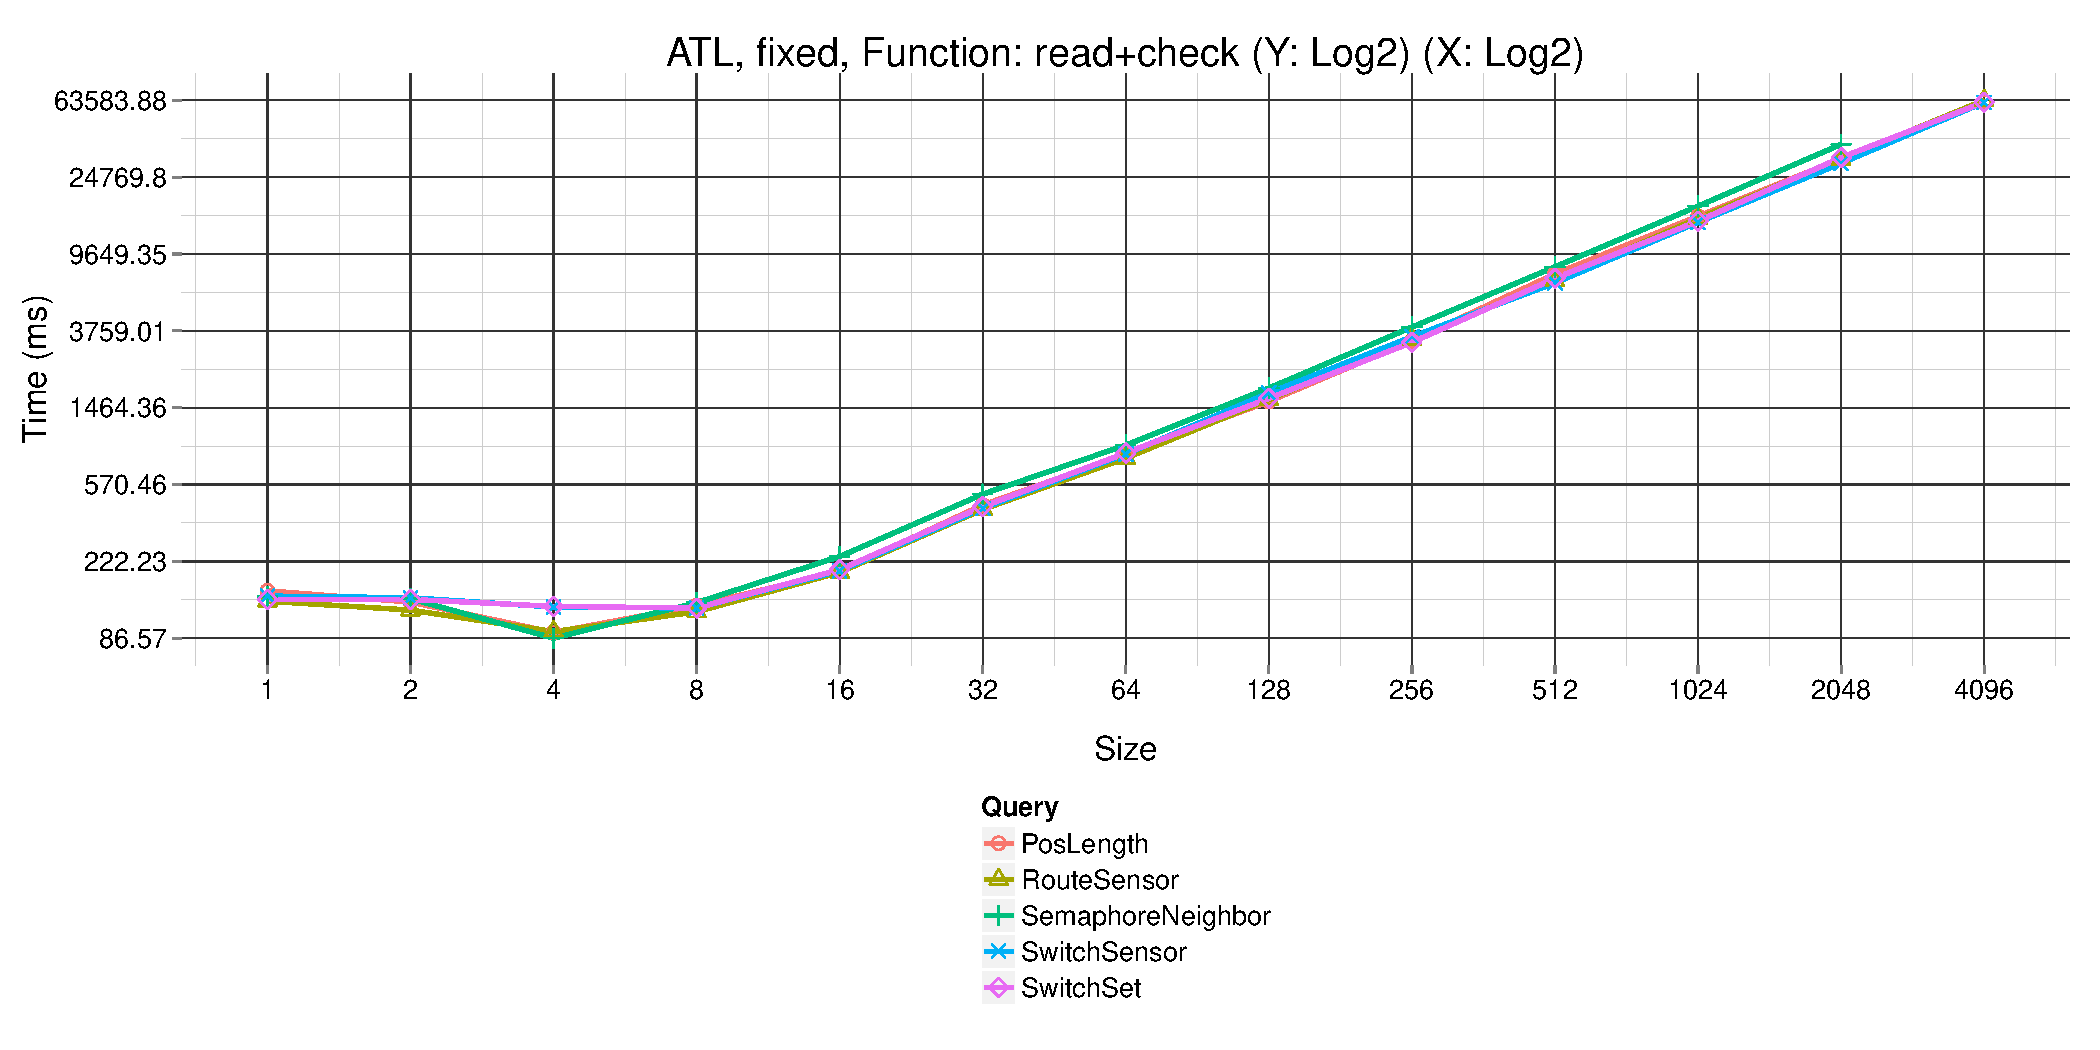
\includegraphics[width=15cm]{figures/fixed-ATL-GroupBy-Query-time-batch-validation}}
\caption{ATL batch validation performance for the fixed scenario}
\label{fig:atl-batch-performance}
\end{figure}

\begin{figure}[ht]
\centerline{
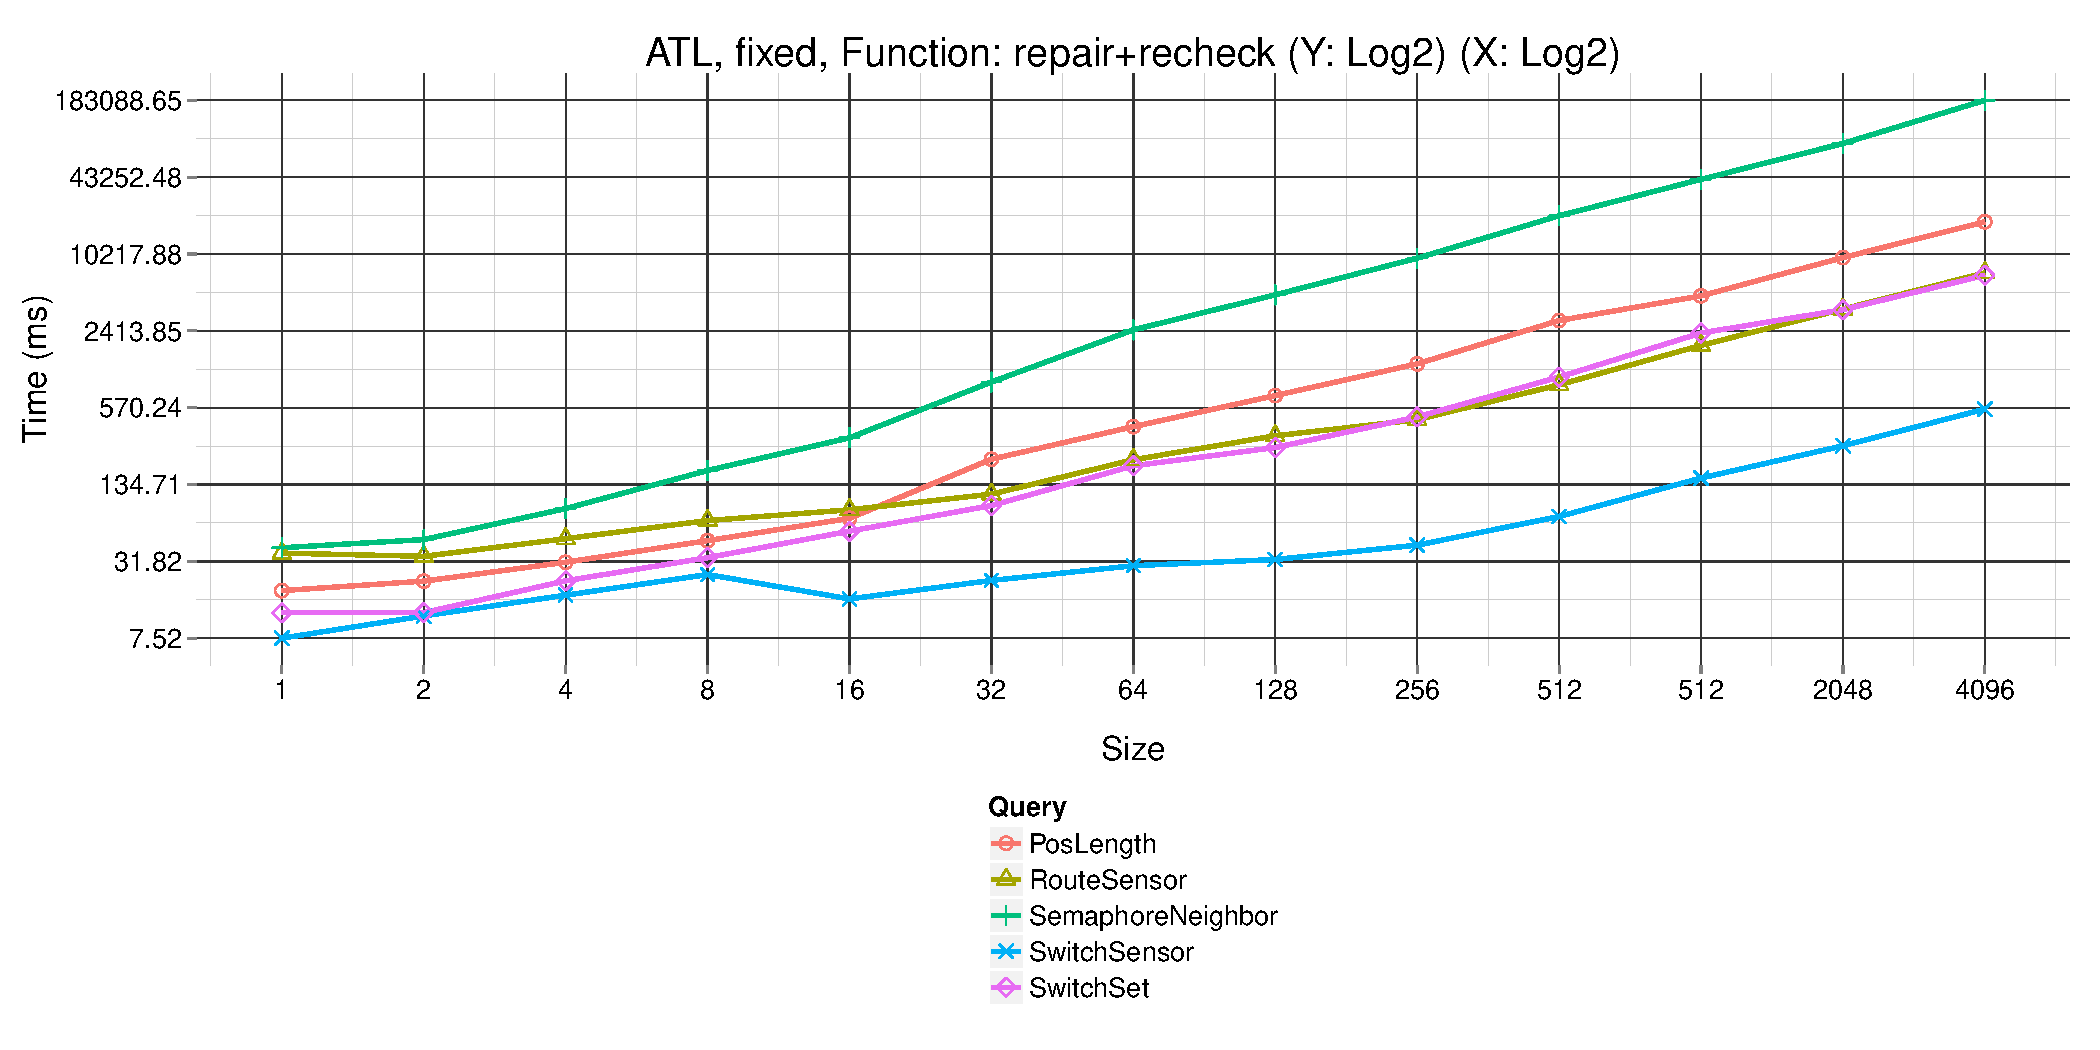
\includegraphics[width=15cm]{figures/fixed-ATL-GroupBy-Query-time-revalidation}}
\caption{ATL revalidation performance for the fixed scenario}
\label{fig:atl-recheck-performance}
\end{figure}


\appendix

\section{Alternative Solution for SemaphoreNeighbor}
\label{appendix:a}

Listing~\ref{lst:semaphoreneighbor} shows an alternative ATL query for SemaphoreNeighbor, using only the ATL language. The query collects the match Tuples for each Route \texttt{r1} with an exit Semaphore, for which there is a Route \texttt{r2} that is different from Route \texttt{r1}, and of which the entry differs from the \texttt{r1} exit, connected to Sensor \texttt{s2}, where \texttt{s2} is connected to Sensor \texttt{s1} or Route \texttt{r1} by TrackElements \texttt{te1} and \texttt{te2}. The resulting nested Collections are flattened into a single Collection of Tuples.

\lstset{language=atl}
\begin{lstlisting}[float=htb, caption={SemaphoreNeighbor query in ATL}, label=lst:semaphoreneighbor, captionpos=b, frame=tb, belowskip=-10pt]
query SemaphoreNeighbour = RAILWAY!Route.allInstances()
	->reject(r1 | r1.exit.oclIsUndefined())
	->collect(r1 | 
		r1.definedBy->collect(s1 | 
			s1.elements->collect(te1 | 
				te1.connectsTo->reject(te2 | 
					let s2 : RAILWAY!Sensor = te2.sensor in
					s2.oclIsUndefined() or not (
					let r2 : RAILWAY!Route = s2.refImmediateComposite() in
					r2.oclIsKindOf(RAILWAY!Route) and r2 <> r1 and r2.entry <> r1.exit)
				)->collect(te2 |
					let s2 : RAILWAY!Sensor = te2.sensor in
					Tuple{s = r1.exit, r1 = r1, r2 = s2.refImmediateComposite(), 
						s1 = s1, s2 = s2, te1 = te1, te2 = te2}
				)
			)
		)
	)->flatten();
\end{lstlisting}

Fig.~\ref{fig:atl-batch-performance-alt} shows the batch read and check scenario performance for the ATL/EMFTVM solution, and Fig.~\ref{fig:atl-recheck-performance-alt} shows the repetitive recheck and repair scenario performance. When comparing these figures to Fig.~\ref{fig:atl-batch-performance} and Fig.~\ref{fig:atl-recheck-performance}, one sees that the performance of this alternative query is consistently worse than the SimpleGT solution. Apparently, the overhead of the OCL collection operations -- many \texttt{collect}s followed by \texttt{flatten} -- makes a big difference. Apart from that, the local search algorithm implemented here in OCL closely resembles what EMFTVM's built in local search engine does. To see the exact difference between the ATL and SimpleGT solution, once has to compare the EMFTVM bytecode of both solutions ("SemaphoreNeighbour.emftvm" for ATL, and "SemaphoreNeighbourCheck.emftvm" for SimpleGT). The Eclipse tooling for ATL/EMFTVM\footnote{\url{http://marketplace.eclipse.org/content/atlemftvm}} includes an EMF-based editor for the bytecode.

\begin{figure}[ht]
\centerline{
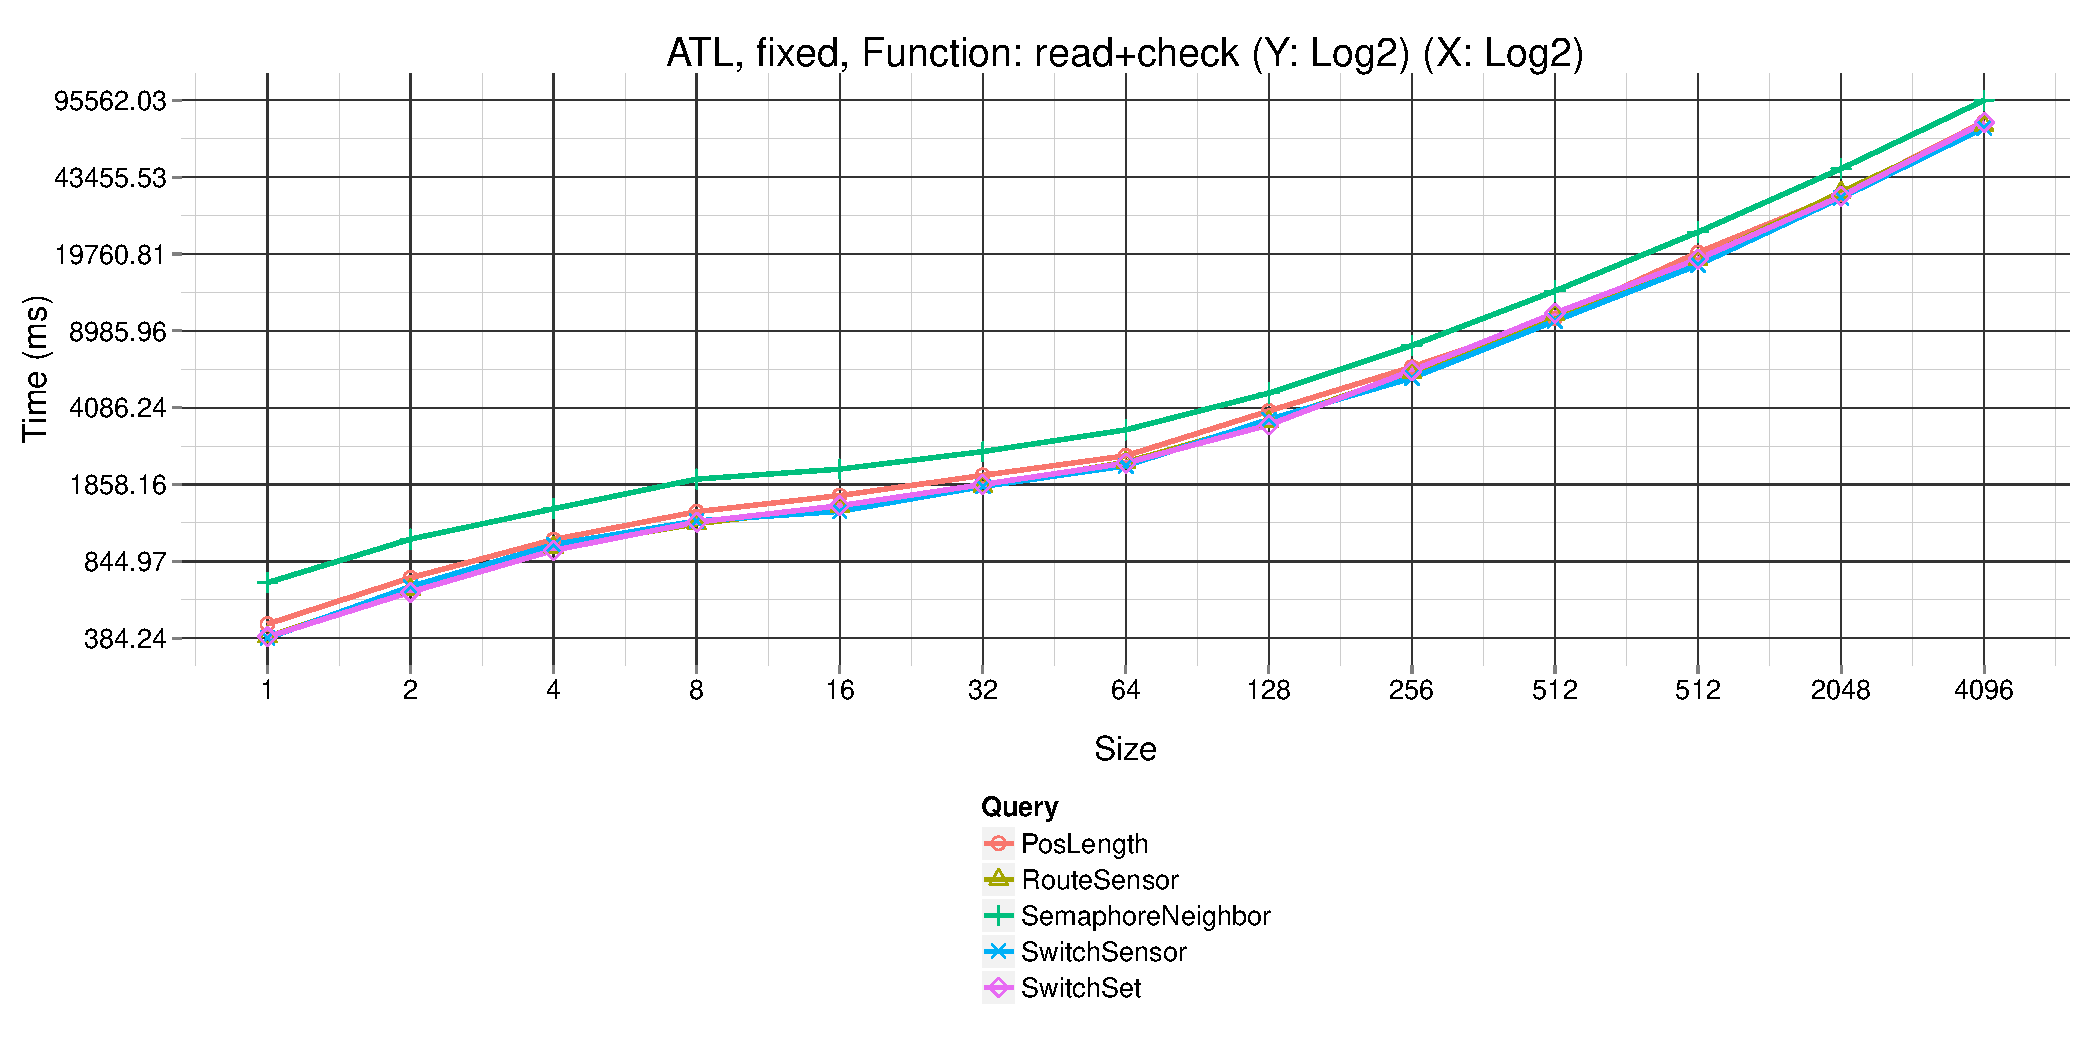
\includegraphics[width=15cm]{figures/fixed-ATL-GroupBy-Query-time-batch-validation-alt}}
\caption{ATL alternative solution batch validation performance for the fixed scenario}
\label{fig:atl-batch-performance-alt}
\end{figure}

\begin{figure}[ht]
\centerline{
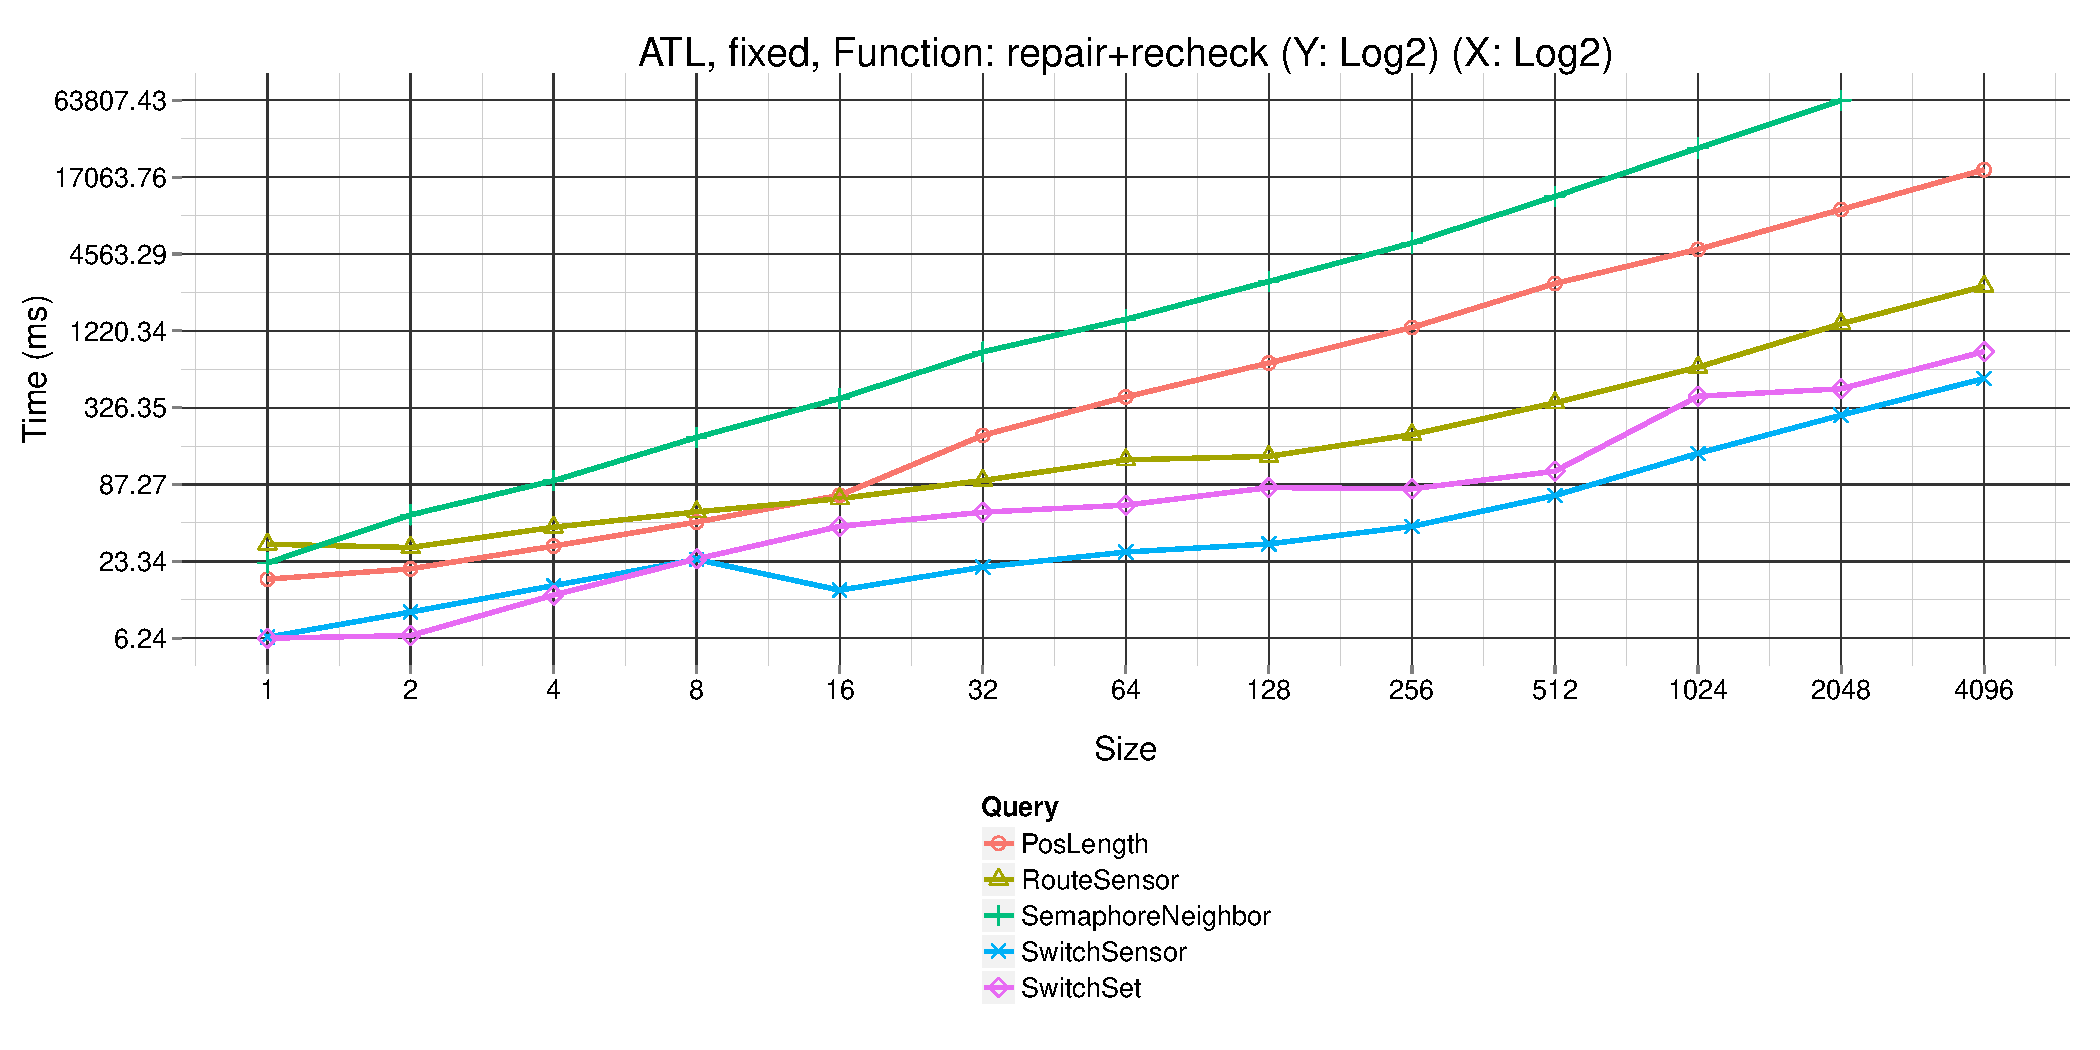
\includegraphics[width=15cm]{figures/fixed-ATL-GroupBy-Query-time-revalidation-alt}}
\caption{ATL alternative solution revalidation performance for the fixed scenario}
\label{fig:atl-recheck-performance-alt}
\end{figure}


\bibliographystyle{eptcs}
\bibliography{ttc15-atl}
\end{document}
